%% LyX 1.3 created this file.  For more info, see http://www.lyx.org/.
%% Do not edit unless you really know what you are doing.
\documentclass[english, 12pt]{article}
\usepackage{times}
%\usepackage{algorithm2e}
\usepackage{url}
\usepackage{bbm}
\usepackage[T1]{fontenc}
\usepackage[latin1]{inputenc}
\usepackage{geometry}
\geometry{verbose,letterpaper,tmargin=2cm,bmargin=2cm,lmargin=1.5cm,rmargin=1.5cm}
\usepackage{rotating}
\usepackage{color}
\usepackage{graphicx}
\usepackage{amsmath, amsthm, amssymb}
\usepackage{setspace}
\usepackage{lineno}
\usepackage{hyperref}
\usepackage{bbm}
\usepackage{makecell}

%\renewcommand{\arraystretch}{1.8}

%\usepackage{xr}
%\externaldocument{paper-ldpred2-supp}

%\linenumbers
%\doublespacing
\onehalfspacing
%\usepackage[authoryear]{natbib}
\usepackage{natbib} \bibpunct{(}{)}{;}{author-year}{}{,}

%Pour les rajouts
\usepackage{color}
\definecolor{trustcolor}{rgb}{0,0,1}

\usepackage{dsfont}
\usepackage[warn]{textcomp}
\usepackage{adjustbox}
\usepackage{multirow}
\usepackage{graphicx}
\graphicspath{{../figures/}}
\DeclareMathOperator*{\argmin}{\arg\!\min}
\usepackage{algorithm} 
\usepackage{algpseudocode} 

\let\tabbeg\tabular
\let\tabend\endtabular
\renewenvironment{tabular}{\begin{adjustbox}{max width=0.9\textwidth}\tabbeg}{\tabend\end{adjustbox}}

\makeatletter

%%%%%%%%%%%%%%%%%%%%%%%%%%%%%% LyX specific LaTeX commands.
%% Bold symbol macro for standard LaTeX users
%\newcommand{\boldsymbol}[1]{\mbox{\boldmath $#1$}}

%% Because html converters don't know tabularnewline
\providecommand{\tabularnewline}{\\}

\usepackage{babel}
\makeatother


\begin{document}


\title{Clarifications on using snpnet and bigstatsr\\ for fitting penalized regressions in very large datasets}
\author{Florian Priv\'e,$^{\text{1,}*}$ Bjarni J. Vilhj\'almsson$^{\text{1,2}}$ and Hugues Aschard$^{\text{3}}$}

\date{~ }
\maketitle

\noindent$^{\text{\sf 1}}$National Centre for Register-Based Research, Aarhus University, Aarhus, 8210, Denmark. \\
\noindent$^{\text{\sf 2}}$Bioinformatics Research Centre, Aarhus University, Aarhus, 8000, Denmark. \\
\noindent$^{\text{\sf 3}}$Centre de Bioinformatique, Biostatistique et Biologie Int\'egrative (C3BI), Institut Pasteur, Paris, 75015, France. \\
\noindent$^\ast$To whom correspondence should be addressed.\\

\noindent Contact:
\begin{itemize}
\item \url{florian.prive.21@gmail.com}
\end{itemize}

\vspace*{4em}

\abstract{	

}


%%%%%%%%%%%%%%%%%%%%%%%%%%%%%%%%%%%%%%%%%%%%%%%%%%%%%%%%%%%%%%%%%%%%%%%%%%%%%%%%

\clearpage

\section*{Introduction}

Penalized regressions such as regression using a lasso penalty has been widely used, as it proved to be a [ ] method for both variable selection and model fitting at the same time \cite[]{tibshirani1996regression}.
R package glmnet is a popular software to fit the lasso efficiently \cite[]{friedman2010regularization}.
However, glmnet cannot handle very large datasets such as biobank-scale data that are now available in human genetics, where both the sample size and the number of variables are very large.
One strategy used to run penalized regressions on such large datasets such as the UK Biobank \cite[]{bycroft2018uk} has been to apply a variable pre-selection step before fitting the lasso \cite[]{lello2018accurate}.
Very recently, authors of the glmnet package have developed a new R package, snpnet, to fit penalized regression on the UK Biobank \cite[]{qian2020fast}.
Before that, we have developed two R packages for efficiently analyzing large-scale data, namely bigstatsr and bigsnpr \cite[]{prive2018efficient}.
We then specifically implemented some highly efficient implementation of penalized regression in R package bigstatsr and showed how this would be useful for genetic prediction with some applications to the UK Biobank \cite[]{prive2019efficient}.
Here, we would like to come back to some statements made in \cite[]{qian2020fast} which we do not find to be always exact.
We reinvestigate the similarities and differences between snpnet and bigstatsr/bigsnpr through some further comparisions and explanations.
We also make more appropriate recommendations on how to fit penalized regressions in the context of genetic data.


%%%%%%%%%%%%%%%%%%%%%%%%%%%%%%%%%%%%%%%%%%%%%%%%%%%%%%%%%%%%%%%%%%%%%%%%%%%%%%%%

\section*{Main motivation for snpnet}

Before we can present the main motivation behind snpnet developed by \cite{qian2020fast}, let us recall how the lasso regression is fitted.
Finally, for penalized logistic regression (PLR), we find regression coefficients $\beta_0$ and $\beta$ that minimize the following regularized loss function 
\begin{equation}
L(\lambda) = \underbrace{ \sum_{i=1}^n \left( y_i - \beta_0 - \sum_{j=1}^p X_{i,j} \beta_j \right)^2 }_\text{Loss function}   +   \underbrace{ \sum_{j=1}^p \lambda |\beta_j| }_\text{Penalization} ~,\label{eq:lasso}
\end{equation}
where $X$ is denoting the matrix composed of $p$ genotypes and possible covariates (e.g.\ sex, age and principal components) for $n$ individuals, $y$ is the (continuous) trait to predict, $\lambda$ ($> 0$) is a regularization hyper-parameter that control the strength of the penalty.
For a sequence of $\lambda$, we can find $\argmin_{\beta} L(\lambda)$ using cyclical coordinate descent\cite[]{friedman2010regularization}.
To speed up the coordinate descent, we can use sequential strong rules for discarding lots of variables (i.e.\ setting lots of $\beta_j$ to $0$) a priori \cite[]{tibshirani2012strong}.
The main drawback of these rules for discarding variants that will not enter the model is that they require a post-phase of checking Karush-Kuhn-Tucker (KKT) conditions.
These conditions are first checked in the ever-active set (set of all variables $j$ with $\beta_j \neq 0$ for any previous $\lambda$). 
Then, the cyclical coordinate descent has to be rerun while adding the new variables that do not satisfy these KKT conditions.
This can happen from time to time
Finally, you have to also check the KKT conditions for all variables in the data.
This last step can be very time consuming for large datasets because it requires to pass over the whole dataset once again.
If the available memory is not large enough to fit the whole dataset, then it means accessing data directly from disk, which is very slow. 

\cite{qian2020fast} have developed a clever approach called batch screening iterative lasso (BASIL) to be able to check these KKT conditions only after having fitted solutions for many $\lambda$, instead of performing this operation for each $\lambda$.
As an example, it can take one hour just to access a large dataset from disk; if you have to do this for 100 different $\lambda$ values, it therefore takes at least 100 hours; but it you can do this only every 5 values of $\lambda$, then it would take only 20 hours instead.
Hence, the BASIL procedure enables to fit the exact lasso solution at a lower computation time for very large datasets.
As bigstatsr is not using this procedure, \cite{qian2020fast} assume that fitting penalized regression with R package bigstatsr should be very slow for large datasets.
We indeed check the KKT conditions for the ever-active set. This set is assumed to be composed of a subset of the total number of variables only, and therefore this is step is fast.
Indeed, what is slow is to test the KKT conditions for the remaining variables. As stated in \cite{tibshirani2012strong} and \cite{qian2020fast}, when $p > n$, KKT conditions for the remaining variables almost always hold. 
Therefore we decided to skip this step when designing functions \texttt{big\_spLinReg} and \texttt{big\_spLogReg} in R package bigstatsr two years ago.
Therefore, these functions effectively access all variables only once at the beginning to compute the statistics used for the strong rules, and then access only a subset of variables (the ever-active set).
As bigstatsr is using memory-mapping, data that resides on disk is accessed only once from disk to memory and then stays in memory while there is no need to free some memory.
Only when the ever-active set becomes large, e.g.\ for very polygenic traits, memory can become an issue, but this extreme case would become a problem for snpnet as well.
Please refer to the Discussion section of \cite{prive2019efficient} for more details on these matters.

To sum up, bigstatsr effectively does less passes on the whole dataset (only one) as compared to snpnet that often does 20 passes or even more.
Moreover, there is a single pass done even when performing cross-validation (CV) internally, while perfoming CV with snpnet would multiply the number of folds used (see next section).

[TALK ABOUT THAT BASIL DOES NOT REALLY DECREASE THE NUMBER OF ITERATIONS FOR HEIGHT?]

%%%%%%%%%%%%%%%%%%%%%%%%%%%%%%%%%%%%%%%%%%%%%%%%%%%%%%%%%%%%%%%%%%%%%%%%%%%%%%%%

\section*{Missing cross-validation?}

In their paper, \cite{qian2020fast} divide the individuals that they use in 60\% for training, 20\% for validation (i.e.\ choosing the best-performing $\lambda$) and 20\% for testing the resulting model.
This is effectively using only 75\% of the data that could be used for training.
Moreover, in the snpnet package, they do not seem to provide any framework for performing cross-validation (CV), as opposed to in R package glmnet.
CV is an inevitable step to fit models with hyper-parameters such as the lasso.
In functions \texttt{big\_spLinReg} and \texttt{big\_spLogReg} of R package bigstatsr, we therefore decided to directly perform a link of cross-validation internally \cite[]{prive2019efficient}.
We divide the training set in $K$ (e.g.\ $10$) sets, which are in turn used as validation set while the others ($K - 1$) sets are used as training set.
Instead of choosing the best performing hyper-parameters and refitting the models using the whole training set, we average the $K$ models because we find it more appropriate and faster, and call this procedure Cross-Model Selection and Averaging (CMSA).
Using CMSA, we are effectively using 100\% of the training set, therefore we expect prediction to be better when using bigstatsr. 
Moreover, because we are using memory-mapping in R package bigstatsr, the data is shared across processes and therefore we can process these folds in parallel without using any extra memory.

%%%%%%%%%%%%%%%%%%%%%%%%%%%%%%%%%%%%%%%%%%%%%%%%%%%%%%%%%%%%%%%%%%%%%%%%%%%%%%%%

\section*{Recommendations}

First, in their UK Biobank applications, \cite{qian2020fast} have tried using elastic-net regularization instead of lasso regression by introducing a new hyper-parameter $\alpha$ ($0 < \alpha \le 1$, with the special case of $\alpha = 1$ being the lasso regularization). 
They show that lasso regularization is very effective in very large (effective) sample sizes, and elastic-net regularization ($\alpha < 1$) might not be needed in this case, which we have also experienced.
Yet, in smaller sample sizes and for very polygenic architectures, we showed through extensive simulations that using lower values for $\alpha$ can significantly improve predictive performance \cite[]{prive2019efficient}.
In \cite{qian2020fast}, they tried $\alpha \in \{0.1, 0.5, 0.9, 1\}$; we recommend to use a grid on the log-scale with smaller values (e.g.\ $1$, $0.1$, $0.01$, $0.001$, and even until $0.0001$).
Note that the smaller is $\alpha$, the larger is the number of non-zero variables and therefore the larger are the time and memory taken by the algorithm.
In functions \texttt{big\_spLinReg} and \texttt{big\_spLogReg} of R package bigstatsr, we allow to directly test many $\alpha$ values in parallel within the CMSA procedure.

Second, for large datasets, one should always use early-stopping.
Indeed, while fitting the regularization path of $\lambda$ values on the training set, one can monitor the predictive ability on the validation step, and stop early in the regularization path when the model starts to overfit the training data and become worse on the validation set (Figure \ref{fig:CMSA}). 
For large data and therefore large validation sets, performances on the validation sets are very smooth and then one can safely stop very early, e.g.\ after the second iteration where prediction becomes worse in the validation set.
This corresponds to setting \texttt{n.abort = 2} in bigstatsr and \texttt{stopping.lag = 2} in snpnet.
This is particularly useful as when we move down the regularization path of $\lambda$ values, more and more variables are entering the model and the cyclical coordinate descent takes more and more time to perform.

\begin{figure}[h]
	\centerline{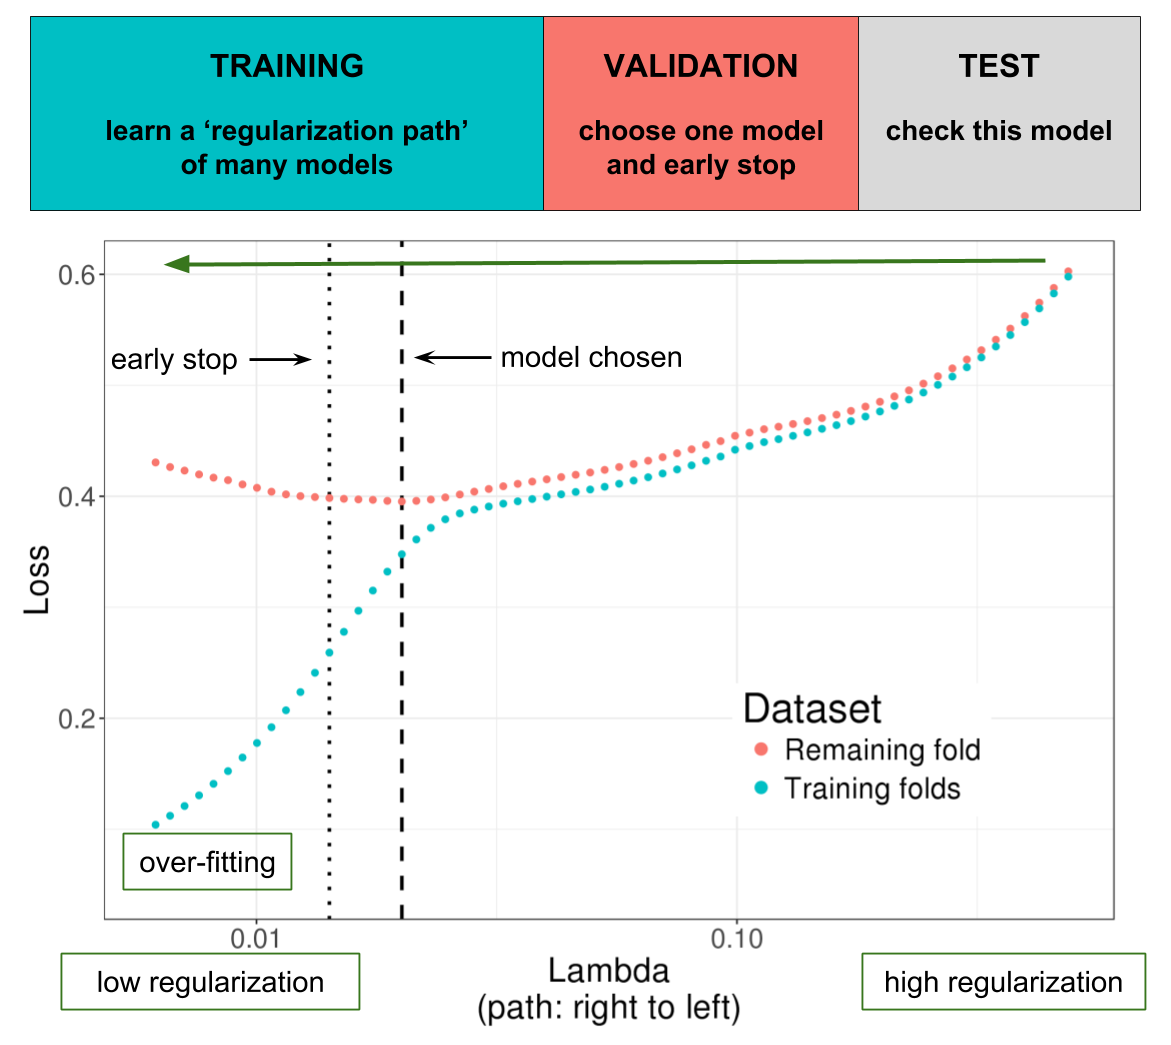
\includegraphics[width=0.85\textwidth]{simple-CMSA}}
	\caption{Illustration of one turn of the Cross-Model Selection and Averaging (CMSA) procedure (figure from \cite{prive2019efficient}). First, this procedure separates the training set in $K$ folds (e.g.\ 10 folds). 
		Secondly, in turn, each fold is considered as an inner validation set (red) and the other ($K - 1$) folds form an inner training set (blue). A ``regularization path'' of models is trained on the inner training set and the corresponding predictions (scores) for the inner validation set are computed. The model that minimizes the loss on the inner validation set is selected. Finally, the $K$ resulting models are averaged. 
		We also use this procedure to derive an early stopping criterion so that the algorithm does not need to evaluate the whole regularization paths, making this procedure much faster.}
	\label{fig:CMSA}
\end{figure}

Third, \cite{qian2020fast} recommend to not scale genotype data to fit lasso. This is both true and false. 
Scaling genotypes is assuming that all variants explain the same amount of variance on average, which is the assumptions behind models in software such as GCTA and LDSC [CITE].
It also means that low-frequency variants would get larger effects on average.
[CITE DOUG] argued that this assumption might not be reasonable and proposed another model [TODO].
In [CITE] they estimated [BLABLA] to be between $-0.25$ and $-0.5$ for most traits.
Note that scaling genotypes by dividing genotypes by their standard deviations as done by default in bigstatsr would correspond to using $-1$ while not doing any scaling as argued by \cite{qian2020fast} would correspond to using $0$.
Therefore, a tradeoff between these two approaches provides higher predictive performance and is therefore recommended (Manuscript in preparation).
For example, in the case of lasso regularization, using a different scaling can be obtained by using a different penalty for all variants, replacing $\lambda$ by different $\lambda_j$ in equation \eqref{eq:lasso}.
This option is available in both bigstatsr and snpnet.

%%%%%%%%%%%%%%%%%%%%%%%%%%%%%%%%%%%%%%%%%%%%%%%%%%%%%%%%%%%%%%%%%%%%%%%%%%%%%%%%

\section*{From theory to practice}

In previous sections, we have explained theoritically why snpnet could not be faster than bigstatsr nor provide higher predictive performance.
In this section, we perform comparisons for 4 traits in the UK Biobank to practically support our claims.

[TODO: SHOWING PREDICTION FOR BOTH THE SAME FOLD AND CMSA + TIMING]

%%%%%%%%%%%%%%%%%%%%%%%%%%%%%%%%%%%%%%%%%%%%%%%%%%%%%%%%%%%%%%%%%%%%%%%%%%%%%%%%

\section*{Conclusion}

[THEY CHOSE THE CLEVER APPROACH, WE CHOSE THE PRACTICAL ONE]

[DISCUSS ABOUT FLEXIBILITY OF THE PACKAGES]


%%%%%%%%%%%%%%%%%%%%%%%%%%%%%%%%%%%%%%%%%%%%%%%%%%%%%%%%%%%%%%%%%%%%%%%%%%%%%%%%

\clearpage
%\vspace*{5em}

\section*{Software and code availability}

[TODO: EXPORT CODE FROM CLUSTER] 

%All code used for this paper is available at \url{https://github.com/privefl/paper-ldpred2/tree/master/code}.
%The newest version of R package bigsnpr can be installed from GitHub (see \url{https://github.com/privefl/bigsnpr}).
%A tutorial on the steps to run LDpred2 using some small example data is available at \url{https://privefl.github.io/bigsnpr/articles/LDpred2.html}. 

\section*{Acknowledgements}

This research has been conducted using the UK Biobank Resource under Application Number 41181.
Authors would also like to thank GenomeDK and Aarhus University for providing computational resources and support that contributed to these research results.

\section*{Funding}

F.P. and B.V.\ are supported by the Danish National Research Foundation (Niels Bohr Professorship to Prof. John McGrath), and also acknowledge the Lundbeck Foundation Initiative for Integrative Psychiatric Research, iPSYCH (R248-2017-2003).

\section*{Declaration of Interests}

The authors declare no competing interests.

%%%%%%%%%%%%%%%%%%%%%%%%%%%%%%%%%%%%%%%%%%%%%%%%%%%%%%%%%%%%%%%%%%%%%%%%%%%%%%%%

\clearpage

\bibliographystyle{natbib}
\bibliography{refs}

%%%%%%%%%%%%%%%%%%%%%%%%%%%%%%%%%%%%%%%%%%%%%%%%%%%%%%%%%%%%%%%%%%%%%%%%%%%%%%%%


\end{document}
